%%%%%%%%%%%%%%%%%%%%%%%%%%%%%%%%%%%%%%%%%
% Short Sectioned Assignment
% LaTeX Template
% Version 1.0 (5/5/12)
%
% This template has been downloaded from:
% http://www.LaTeXTemplates.com
%
% Original author:
% Frits Wenneker (http://www.howtotex.com)
%
% License:
% CC BY-NC-SA 3.0 (http://creativecommons.org/licenses/by-nc-sa/3.0/)
%
%%%%%%%%%%%%%%%%%%%%%%%%%%%%%%%%%%%%%%%%%

%----------------------------------------------------------------------------------------
%	PACKAGES AND OTHER DOCUMENT CONFIGURATIONS
%----------------------------------------------------------------------------------------

\documentclass[letterpaper, fontsize=11pt]{scrartcl} % A4 paper and 11pt font size

\usepackage[T1]{fontenc} % Use 8-bit encoding that has 256 glyphs
\usepackage{fourier} % Use the Adobe Utopia font for the document - comment this line to return to the LaTeX default
\usepackage[english]{babel} % English language/hyphenation
\usepackage{amsmath,amsfonts,amsthm} % Math packages

\usepackage{lipsum} % Used for inserting dummy 'Lorem ipsum' text into the template
\usepackage[margin=1in]{geometry} %set margins -TA
\usepackage{sectsty} % Allows customizing section commands
\allsectionsfont{\centering \normalfont\scshape} % Make all sections centered, the default font and small caps
\usepackage{enumitem}
\usepackage{fancyhdr} % Custom headers and footers
\usepackage{graphicx}
\pagestyle{fancyplain} % Makes all pages in the document conform to the custom headers and footers
\fancyhead{} % No page header - if you want one, create it in the same way as the footers below
\fancyfoot[L]{\textit{CME 102 Spring '15-'16}} % Empty left footer
\fancyfoot[C]{} % Empty center footer
\fancyfoot[R]{Tim Anderson} % Page numbering for right footer
\renewcommand{\headrulewidth}{0pt} % Remove header underlines
\renewcommand{\footrulewidth}{0pt} % Remove footer underlines
\setlength{\headheight}{14pt} % Customize the height of the header

\numberwithin{equation}{section} % Number equations within sections (i.e. 1.1, 1.2, 2.1, 2.2 instead of 1, 2, 3, 4)
\numberwithin{figure}{section} % Number figures within sections (i.e. 1.1, 1.2, 2.1, 2.2 instead of 1, 2, 3, 4)
\numberwithin{table}{section} % Number tables within sections (i.e. 1.1, 1.2, 2.1, 2.2 instead of 1, 2, 3, 4)

\setlength\parindent{0pt} % Removes all indentation from paragraphs - comment this line for an assignment with lots of text
\begin{document}

%----------------------------------------------------------------------------------------
%	TITLE SECTION
%----------------------------------------------------------------------------------------

\newcommand{\horrule}[1]{\rule{\linewidth}{#1}} % Create horizontal rule command with 1 argument of height

%----------------------------------------------------------------------------------------
%	PROBLEM 1
%----------------------------------------------------------------------------------------

\section*{Week 8 Section Solutions}
\par If not otherwise specified, solve the following problems. If initial conditions are given, solve for all constants of integration. It is okay to leave answers in implicit form or with unsolved integrals. 
\begin{enumerate}
\item For the following, give the natural frequency \textit{$\omega_0$}. State whether or not there is resonance or beats, and give a reason for why.
\begin{enumerate}
\item $y'' + 4y = sin(2t)$ \newline
\textbf{Solution:} 
The homogeneous equation is $y'' + 4y = 0 $ or $ y'' = -4y$.
Then the natural frequency is $\omega_0 = 2$ since our ODE is of the form $y'' = -\omega^2y$. This matches the frequency of the forcing term (the right hand side), so our particular solution is of the form $y_p(t) = Atsin(2t) + Btcos(2t)$ which grows in time. So, we have \underline{resonance}. 
\item $y'' + 2y' + 5y = cos(2t)$ \newline
\textbf{Solution:} 
The homogeneous equation is $y'' + 5y' + 2y = 0 $ which has roots $\lambda = -1 \pm 2i$, so the natural frequency is $\omega_0 = 2$. This matches the frequency of the forcing term (the right hand side). If this were an undamped system, we would have resonance. However, the system is damped and thus will not blow up, so we have neither beats nor resonance.
\item $y'' + y' + 2y = 3$ \newline
\textbf{Solution:} 
he homogeneous equation is $y'' + y' + 2y = 0 $ which has roots $\lambda = -1/2 \pm i\sqrt{7}/2$, so the natural frequency is $\omega_0 = \sqrt{7}/2$. The forcing term is not periodic, so we do not have beats or resonance.  
\item $y'' + 4y = sin(2.05t)$ \newline
\textbf{Solution:} 
The homogeneous problem is the same as in 1(a), and the natural frequency is $\omega_0 = 2$. The forcing term has frequency $\omega = 2.05$, so $\omega_0 \approx \omega$ and we have \underline{beats}. 
\end{enumerate}

\item For the system described by the image below, derive the system of ODEs governing the mass-spring system. Treat the masses as point masses and assume no damping or friction.
\newline
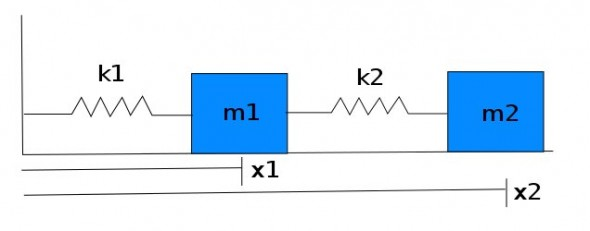
\includegraphics[width=5in]{section8_1.jpg}
\newline
Derive the system of ODEs governing the mass-spring system. Treat the masses as point masses and assume no damping or friction. \newline
\textbf{Solution}
$$m_1x_1'' = -(k_1 + k_2)x_1 + k_2x_2$$ 
$$m_2x_2'' = k_2x_1 - k_2x_2$$
Which in matrix form is: $\left[ \begin{array}{c} x_1'' \\ x_2'' \end{array} \right]= \begin{bmatrix} \frac{-(k_1 + k_2)}{m_1} & \frac{k_2}{m_1} \\ \frac{k_2}{m_2} & \frac{-k_2}{m_2} \end{bmatrix} \left[ \begin{array}{c} x_1 \\ x_2 \end{array} \right] $%\left[ \begin{array}{c} x_1'' \\ x_2'' \end{array} \right] 

\item Perform the following integrals:
\begin{enumerate}
\item $\int_{0}^{\infty}e^{-sx} dx$ \newline
\textbf{Solution} \newline
$$\int_{0}^{\infty}e^{-sx} dx =  \frac{-1}{s} e^{-sx} \bigg{|}_0^\infty = 0 - (\frac{-1}{s})  = \frac{1}{s}$$
\item $\int_{0}^{\infty}sin(x)e^{-sx} dx$ \newline
\textbf{Solution} \newline
With integration by parts: 
$$u = sin(x) \text{ , } dv = e^{-sx}$$
$$du = cos(x) \text{ and } v = \frac{-1}{s}e^{-sx}$$
$$\int_{0}^{\infty}sin(x)e^{-sx} dx =sin(x)e^{-sx} - \int_{0}^{\infty}\frac{-1}{s}e^{-sx}cos(x) dx $$
Doing this again for the second integral:
$$u = cos x \text{ , } dv = e^{-sx}$$
$$du = - sin x \text{ and } v = \frac{-1}{s}e^{-sx} $$
$$\int_{0}^{\infty}cos(x)e^{-sx} dx =cos(x)e^{-sx} - \int_{0}^{\infty}\frac{-1}{s}e^{-sx}cos(x) dx $$
And then finally:
$$\int_{0}^{\infty}sin(x)e^{-sx} dx = \frac{ e^{-sx}((s)sin(x) - cos(x))}{s^2 + 1} \bigg{|}_0^\infty = \frac{1}{s^2 + 1}$$

\item $\int_{0}^{\infty}u(x-2)sin(x-2)e^{-sx} dx$ \newline
\textbf{Solution} \newline
Use the substitution $\tau = x -2$, then the integral becomes:
$$\int_{0}^{\infty}u(x-2)sin(x-2)e^{-sx} dx = \int_{0}^{\infty}u(\tau)sin(\tau)e^{-s(\tau + 2)}dx = \int_{0}^{\infty}sin(\tau)e^{-s(\tau + 2)}dx = $$ $$\int_{0}^{\infty}sin(\tau)e^{-s\tau}e^{-2s}d\tau = e^{-2s}\int_{0}^{\infty}sin(\tau)e^{-s\tau}d\tau$$
The integral is the same as in 3(b), so the answer is then:
$$\int_{0}^{\infty}sin(x-2)e^{-sx} dx =  \frac{e^{-2s}}{s^2 + 1}$$

\end{enumerate}

\item Solve the following using a Laplace transform: $$y'' - 2y' +y = 2 \; ; \qquad y(0) = 0 \qquad y'(0) = 0$$
\textbf{Solution} \newline
Taking the Laplace Transform of each side:
$$s^2Y(s) -sy(0) - y'(0) -2(sY(s) - y(0)) +Y(s) = \frac{2}{s}$$
Applying initial conditions:
$$s^2Y(s) -2sY(s) + Y(s) = \frac{2}{s}$$
$$Y(s) =  \frac{2}{s(s^2 - 2s +1)} =  \frac{1}{s} - \frac{1}{s-1} + \frac{1}{(s-1)^2}$$
$$y(t) = 1 - e^t + te^t$$


\end{enumerate}

%----------------------------------------------------------------------------------------

\end{document}